\chapter{Methodology}
\label{chap:methodology}

\section{Technologies Used}
\label{sec:technologies_used}

\begin{enumerate}
    \item \textbf{Knowledge Distillation:} This is the core strategic technique upon which this project is built. It aims to resolve the conflict between the high accuracy of large models and the computational requirements of resource-constrained devices like mobile phones. The fundamental idea is to train a small, efficient model (the "student model") to mimic the behavior and outputs of a large, high-performance model (the "teacher model") \cite{hu2023teacher}.
    \item \textbf{Model Architecture (Encoder-Decoder):} The model is built upon an encoder-decoder architecture, which is a common design for neural networks used for tasks such as depth estimation. The encoder processes the image to extract features, and the decoder then uses these features to generate the depth map.
    \item \textbf{Vision Transformer (ViT):} This is a neural network architecture that is particularly effective at capturing the global context of an image. The teacher model, \textbf{Depth Anything V2}, is based on this technology.
\end{enumerate}

\section{Knowledge Distillation Technique}
\label{sec:kd_technique}

Knowledge Distillation is a form of \textbf{Model Compression} in Machine Learning \cite{hinton2015distilling}. It aims to transfer "knowledge" from a large, complex, high-performance "teacher" model to a smaller, more computationally efficient "student" model. The idea is inspired by the real-world teacher-student relationship, where a teacher not only gives the student the final answer but also explains the thinking and logic that lead to it. The primary objective is to create a compact model with a small memory footprint and fast inference speed, making it suitable for deployment on mobile devices.

\subsection{Distillation Mechanism}
\label{subsec:distillation_mechanism}

The distillation mechanism relies on training the student model not only on the original labeled data ("hard targets") but also on the outputs of the teacher model. The power of this technique lies in the fact that the teacher model provides richer training signals than just the correct answer alone \cite{hu2023teacher}.

\begin{enumerate}
    \item \textbf{Hard Targets:} These are the correct, ground-truth labels from the dataset (e.g., this image contains a cat). Training a small student model exclusively on hard targets can be challenging, as the model may lack the capacity to learn the complex underlying function perfectly.
    \item \textbf{Soft Targets:} These are the complete probabilistic outputs of the teacher model. For example, in a simple classification problem, instead of saying "this is a cat," the teacher might say, "this is 90\% a cat, 6\% a dog, 4\% a rabbit, etc." This probability distribution, known as \textbf{"dark knowledge,"} contains rich, implicit information about the similarity between different classes from the teacher's perspective. When the student learns to mimic these "soft targets," it learns the relational structure between classes, leading to better generalization and higher performance.
\end{enumerate}

\subsection{Types of Distillable Knowledge}
\label{subsec:types_of_knowledge}

The process of distillation is not limited to the final output layer. Multiple types of knowledge can be transferred to enhance the student's performance \cite{hu2023teacher}:
\begin{itemize}
    \item \textbf{Response-Based Distillation:} This is the classic form of distillation, where the student model is trained to directly mimic the final prediction ("soft targets") of the teacher model.
    \item \textbf{Feature-Based Distillation:} In this type, the student model is trained to replicate the intermediate feature maps produced by the teacher's hidden layers. This forces the student to learn the same feature-extraction hierarchy that the teacher uses, helping it to understand the data more deeply.
    \item \textbf{Relation-Based Distillation:} This approach focuses on distilling the relationships between data points or feature maps, such as by having the student model mimic the teacher's attention maps or the correlation matrices between features.
\end{itemize}

\section{Training Methodology}
\label{sec:training_methodology}

The training approach is based on a teacher-student framework to distill and compress the knowledge from the large model to the smaller one.

\begin{itemize}
    \item \textbf{Teacher Model:} The \textbf{Depth Anything V2 (Small)} model is used as the teacher. This model is pre-trained on a massive dataset and produces high-quality depth estimation results, but its large size and computational requirements make it unsuitable for mobile devices.
    \item \textbf{Student Model:} A new, lightweight student model was designed with an architecture such as \textbf{MobileViT-XS}. Its architecture was chosen to have a low parameter count, enabling fast and efficient inference.
\end{itemize}

The distillation process is guided by training the student model to minimize a composite \textbf{Loss Function}. In our case, the loss function consists of four components:

\begin{enumerate}
    \item \textbf{Scale-Invariant Logarithmic Loss (SILog):} This is the primary component, which measures the accuracy of the student's predicted depth map ($d$) compared to the teacher's output ($d^*$). This loss uses a scale-invariant logarithmic scale to ensure structural correctness \cite{eigen2014depth}.
    
    The loss is calculated using the following formula:
    \begin{equation}
        L_{\text{silog}} = \frac{1}{N}\sum_{i} (\log(d_i) - \log(d_i^*))^2 - \frac{1}{N^2} (\sum_{i} (\log(d_i) - \log(d^*_i)))^2
        \label{eq:silog}
    \end{equation}
    
    where $d_i$ and $d_i^*$ are the predicted and teacher depths for each pixel $i$, and $N$ is the total number of pixels. This loss ensures that the structure of the predicted depth map is correct, regardless of the overall scale.  Demonstrated in Figure~\ref{fig:silog_diagram}

    \begin{figure}[htbp]
        \centering
        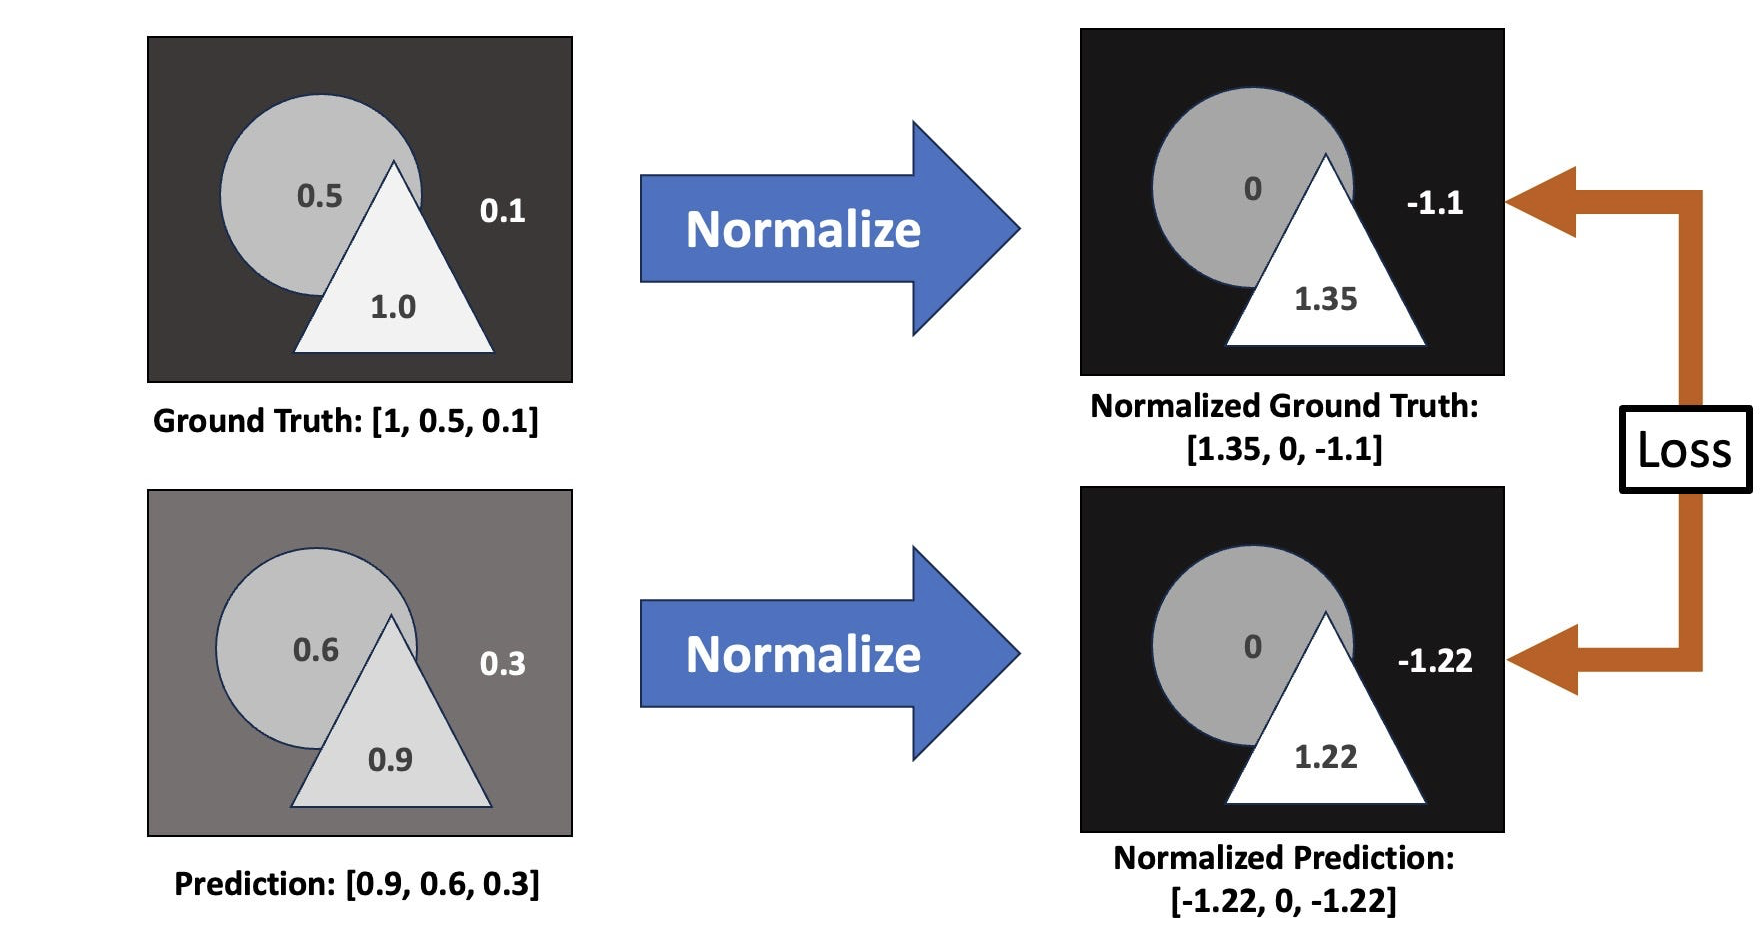
\includegraphics[width=0.8\textwidth]{images/silog_diagram.png}
        \caption{Scale-Invariant Logarithmic Loss.}
        \label{fig:silog_diagram}
    \end{figure}

    \item \textbf{Gradient Matching Loss:} This loss component forces the gradients of the student's depth map to be similar to the gradients of the teacher's depth map. This is crucial for preserving the edges and fine-grained details of the scene \cite{li2018megadepth}.
    
    The loss is calculated as the L1 distance between the teacher and student gradients:
    \begin{equation}
        L_{\text{grad}} = \frac{1}{N} \sum_i \left( |\nabla_x(d_i) - \nabla_x(d_i^*)| + |\nabla_y(d_i) - \nabla_y(d_i^*)| \right)
        \label{eq:grad_loss}
    \end{equation}
    where $d_i$ is the student's prediction, $d_i^*$ is the teacher's prediction, $\nabla_x$ and $\nabla_y$ are the gradient operators (e.g., Sobel filters) in the horizontal and vertical directions  (demonstrated in Figure~\ref{fig:gradient_loss_diagram}), and $N$ is the total number of pixels.

    \begin{figure}[htbp]
        \centering
        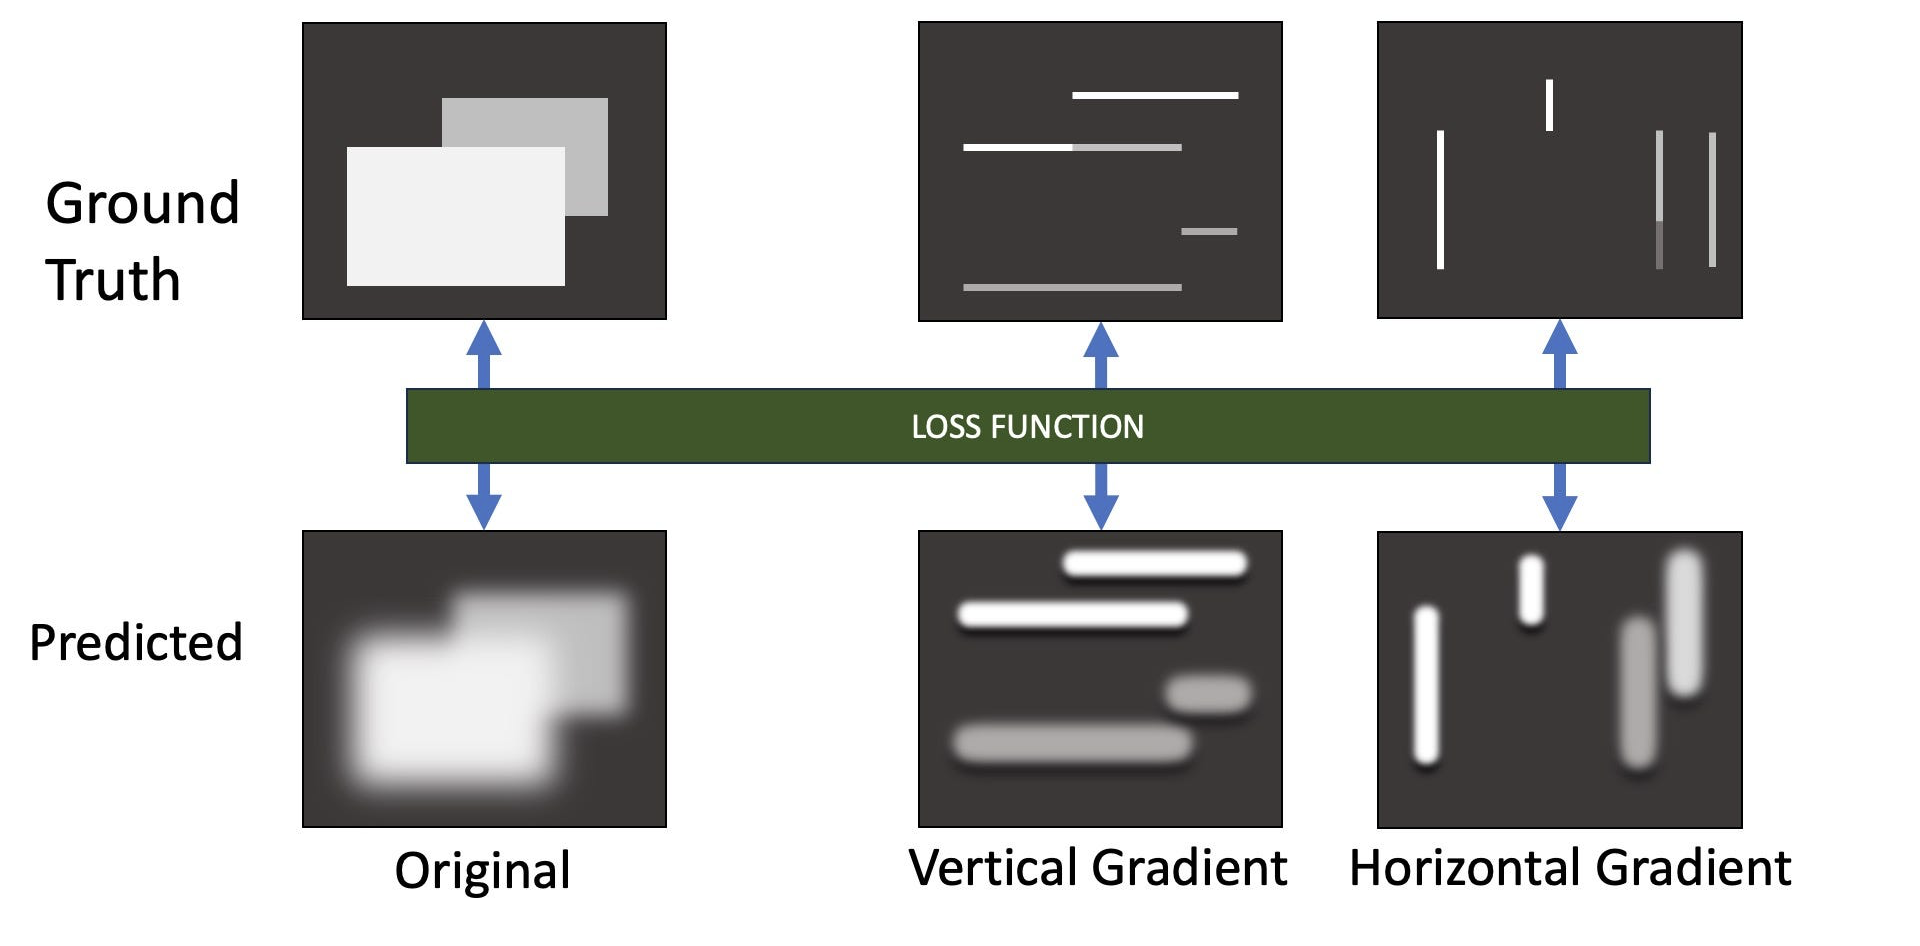
\includegraphics[width=\textwidth]{images/gradient_loss_diagram.png}
        \caption{Gradient Matching Loss.}
        \label{fig:gradient_loss_diagram}
    \end{figure}

    \item \textbf{Feature Matching Loss:} Instead of only mimicking the final output, this loss aims to make the student's intermediate feature maps ($f_i^S$) similar to the teacher's ($f_i^T$). This helps the student learn the "internal representations" that the teacher uses to understand the scene~\cite{hu2023teacher}.
    \begin{equation}
        L_{\text{feat}} = \frac{1}{M} \sum_{i} |f_i^S - f_i^T|
        \label{eq:feat_loss}
    \end{equation}
    where $M$ is the number of features in the feature maps.

    \item \textbf{Attention Matching Loss:} This loss computes a simplified "attention map" for both the student ($attn^S$) and the teacher ($attn^T$) by summarizing their feature maps. By matching these maps, the student is encouraged to focus on the same important spatial regions in the image as the teacher~\cite{hu2023teacher}.
    
    The attention map is generated efficiently and directly by summarizing information across the channel dimension of a feature map. The process is as follows:
    \begin{enumerate}
        \item \textbf{Calculate Absolute Value:} First, the absolute value of all values in the feature map is taken. This ensures that strong activations, whether positive or negative, contribute positively to identifying regions of interest.
        \item \textbf{Average Across Channels:} Next, the average of the values is computed across the channel dimension for each spatial location. This "compresses" the multiple feature maps into a single 2D map representing the relative spatial importance of each region.
    \end{enumerate}
    
    Mathematically, the value of a pixel in the final attention map $attn$ at spatial location $(i,j)$ can be expressed as follows, where $f_{c,i,j}$ is the pixel value in channel $c$ at location $(i,j)$ and $C$ is the total number of channels:
    \begin{equation}
        attn_{i,j} = \frac{1}{C}\sum_{c=1}^{C}|f_{c,i,j}|
    \end{equation}
    
    The loss is then calculated as:
    \begin{equation}
        L_{\text{attn}} = \frac{1}{M'}\sum_{i}(attn^S - attn^T)^2
        \label{eq:attn_loss}
    \end{equation}
\end{enumerate}

These losses are combined into a single total loss function using weighting coefficients ($\lambda$) for each component:
\begin{equation}
    L_{\text{total}} = \lambda_{\text{silog}}L_{\text{silog}} + \lambda_{\text{grad}}L_{\text{grad}} + \lambda_{\text{feat}}L_{\text{feat}} + \lambda_{\text{attn}}L_{\text{attn}}
    \label{eq:total_loss}
\end{equation}
The weighting coefficients will be tuned during practical implementation based on experimental results.

\section{The Student Model (Delta) Design}
\label{sec:delta_model_design}

Several models were designed and tested by changing the encoder or the decoder structure, but we will only describe the final adopted model. The design and development of the student model, named \textbf{Delta ($\Delta$)}, was an iterative process of experimentation and refinement to achieve the best balance between performance and efficiency.

\subsection{Teacher Model Architecture}
\label{subsec:teacher_arch}

The teacher model is \textbf{Depth Anything V2}, which is based on a \textbf{Vision Transformer (ViT)} architecture, specifically \textbf{DINOv2}, The Figure~\ref{fig:teacher_arch} shows the Depth Anything architecture. This model excels at extracting rich and contextual features from the entire image, giving it superior accuracy in depth estimation. It consists of a large ViT-based encoder and a subsequent set of decoder layers that transform these features into a depth map~\cite{yang2024depth,yang2024depthV2}. Its large size makes it impractical for mobile applications. It is worth noting that any inaccuracies in the teacher model's predictions can be propagated to the student during training.

\begin{figure}[htbp!]
    \centering
    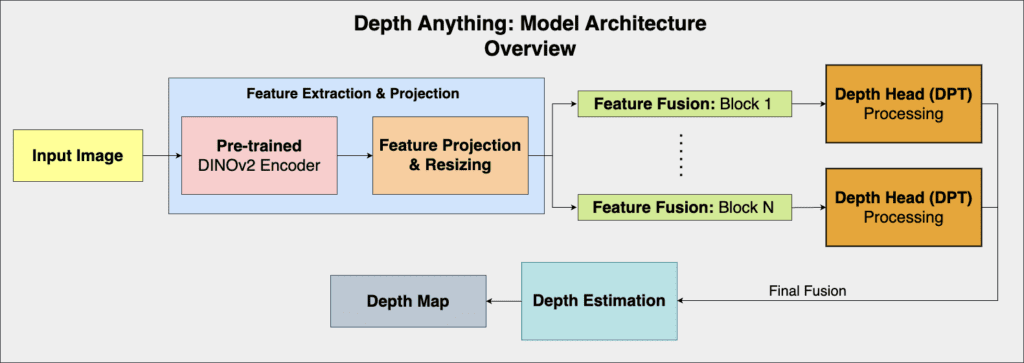
\includegraphics[width=\textwidth]{images/teacher_model_arch.png}
    \caption{Teacher Model Architecture.}
    \label{fig:teacher_arch}
\end{figure}

\subsection{Student Model (Delta) Architecture}
\label{subsec:student_arch}

The student model was designed to achieve a balance between accuracy and inference speed on mobile devices. Taking into consideration that for knowledge distillation, it is often beneficial to design a student architecture that mimics the teacher's structure, the student consists of two main parts (As shown in Figure \ref{fig:delta_arch}):

\begin{enumerate}
    \item \textbf{The Encoder:} The \textbf{MobileViT-XS} architecture was chosen as the encoder for the student model. MobileViT is a hybrid model that combines the efficiency of Convolutional Neural Networks (CNNs) in extracting local features with the ability of Vision Transformers to understand the global context of the image. This architecture makes it lightweight, fast, and ideal for running on mobile phones. The version pre-trained on the ImageNet dataset was used to extract basic features~\cite{mehta2021mobilevit}.

    \item \textbf{The Decoder:} A custom, lightweight decoder module, named \textbf{MiniDPT}, was designed. It is inspired by the DPT architecture~\cite{ranftl2021vision} but with significant simplifications to reduce computational complexity. The decoder receives multi-scale feature maps from the encoder and progressively fuses them to produce the final depth map. This process occurs in three stages:

    \begin{description}
        \item[Projection Stage:] Before fusion begins, each feature map coming from the encoder is processed separately. A \texttt{1x1 convolution}, followed by \texttt{Batch Norm} and a \texttt{ReLU} activation, is applied to each feature map. The goal of this stage is to unify the number of channels across the encoder's feature maps to match the required dimensions for each stage of the decoder.

        \item[Upsampling \& Fusion Stage:] This is the core stage of the decoder. It is an iterative process, starting from the feature map with the lowest spatial resolution (most abstract) and progressing to the highest resolution. In each step of the iteration, two main blocks are applied:
        \begin{enumerate}
            \item \textbf{Upsample Block:} This block is responsible for increasing the spatial resolution. It uses an \texttt{nn.Upsample} layer with bilinear interpolation to double the map's dimensions. Then, for high computational efficiency, the upsampled features are processed using \textbf{Depthwise Separable Convolutions} instead of traditional convolutions. This design choice is crucial for reducing the number of parameters and making the model lightweight.
            \item \textbf{Fusion Block:} This block implements a skip-connection mechanism. It fuses the output from the Upsample Block with the corresponding feature map coming from the "Projection Stage". The fusion is performed via concatenation (\texttt{torch.cat}) along the channel dimension, followed by a series of convolutional layers (\texttt{1x1 Conv}, \texttt{Batch Norm}, \texttt{ReLU}) to process and refine the combined features.
        \end{enumerate}
        This gradual fusion allows the model to combine high-level semantic information from deep layers with fine spatial details from shallow layers.

        \item[Prediction Head:] After the final fusion stage, the resulting feature map is processed through a series of layers to generate the final output. The prediction head consists of \texttt{Conv2d} layers, \texttt{ReLU}, and a final \texttt{Upsample} layer, ending with a \texttt{Conv2d} layer with a kernel size of 1 to produce a single-channel map. A \texttt{Sigmoid} activation function is then applied to ensure the output depth values are normalized between 0 and 1.
    \end{description}
\end{enumerate}

The final student model consists of \textbf{3,373,265} parameters (~3.4 million). In comparison, the teacher model has \textbf{24.8 million} parameters, making our student model approximately \textbf{1/7th} the size of the teacher model.


\begin{figure}[htbp!]
    \centering
    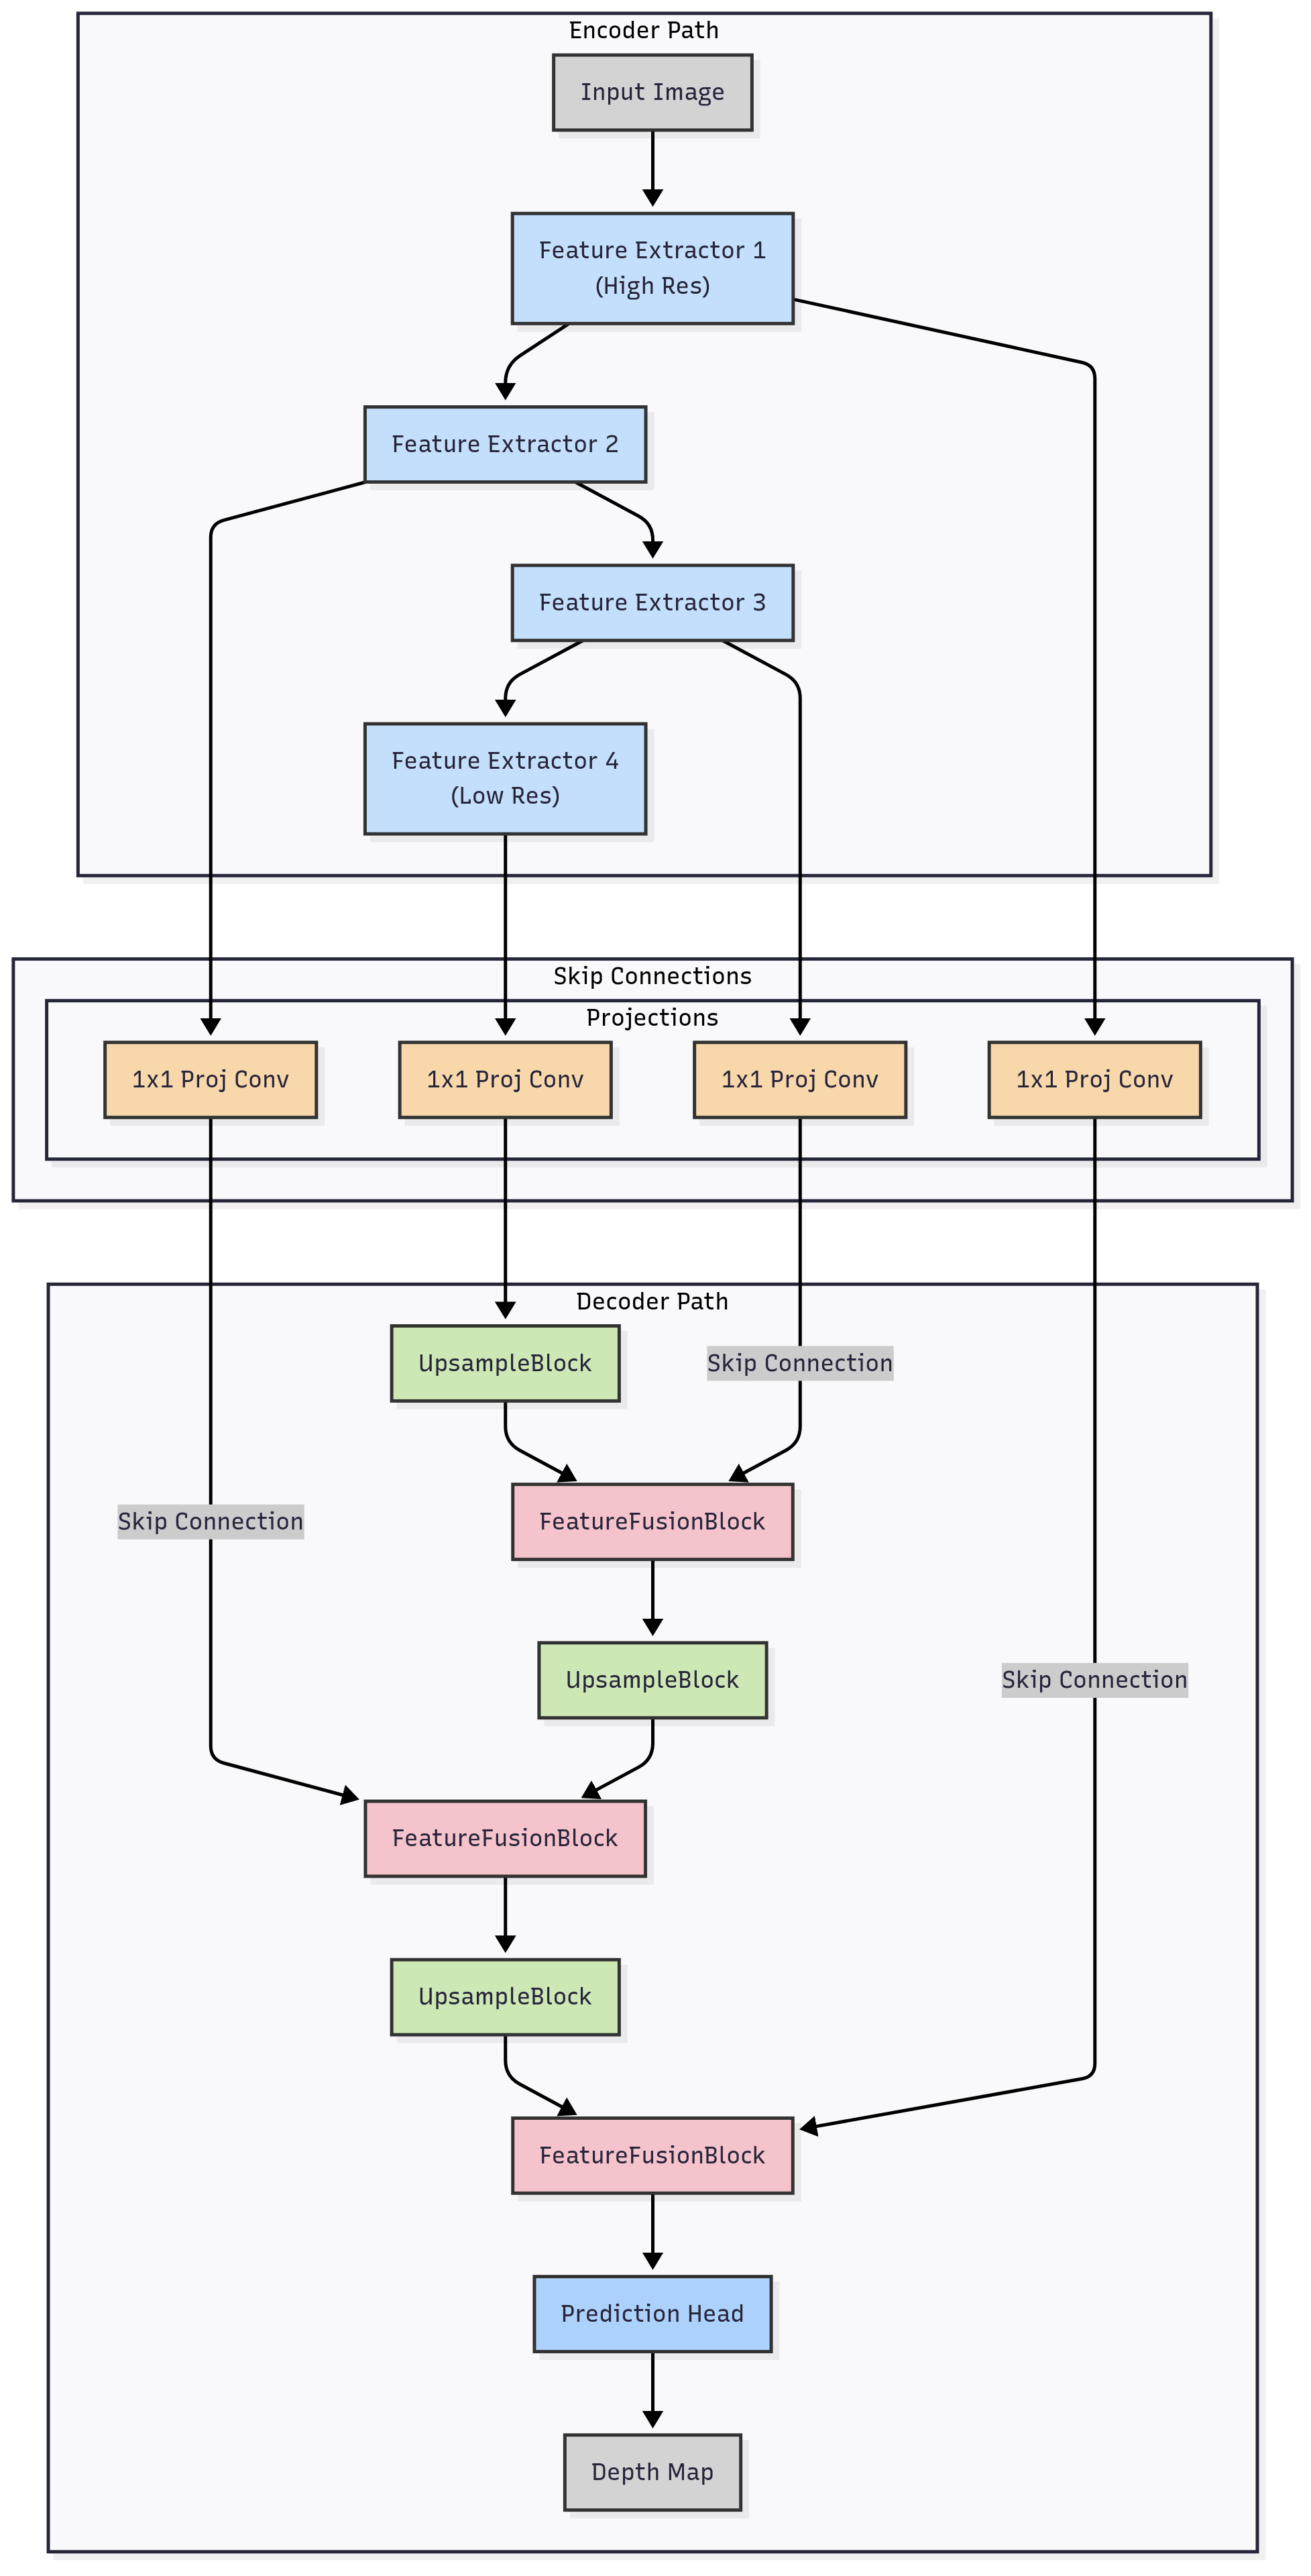
\includegraphics[width=0.9\textwidth, height=0.9\textheight]{images/delta_arch.png}
    \caption{Student Model (Delta) Architecture}
    \label{fig:delta_arch}
\end{figure}